\chapter{Move Generation}
\label{move generation} %\label{1cap:spinta_laterale}
% [titolo ridotto se non ci dovesse stare] {titolo completo}
%


\newpage


\section{Introduzione} %\label{1sec:scopo}
Una volta stabilito il tipo di rappresentazione il passo successivo è quello della generazione delle mosse,per generazione delle mosse si intende la generazione
di tutte le mosse legali eseguibili data una posizione di partenza , la generazione delle mosse è un processo fondamentale in quanto identifica i rami che
il nostro algoritmo potrà esplorare nella successiva fase, quella appunto di ricerca, trattata nel capitolo \ref{ricerca}.





\section{approcci alla generazione delle mosse}
Una volta stabilito il tipo di rappresentazione il passo successivo è quello della generazione delle mosse,per generazione delle mosse si intende la generazione
di tutte le mosse legali eseguibili data una posizione di partenza , la generazione delle mosse è un processo fondamentale in quanto identifica i rami che
il nostro algoritmo potrà esplorare nella successiva fase, quella appunto di ricerca, trattata nel capitolo \ref{ricerca}.
La generazione delle mosse viene affrontata con 3 approcci radicalmente diversi a seconda del tipo di pezzo che stiamo trattando,in particolare la distinzione si effettua tra 
pedoni,pezzi scorrevoli (alfieri,torri,regine) e non scorrevoli(re e cavalli).

\subsection{pedoni}
Il pedone muove solo in avanti, mai indietro o di lato. Un pedone può avanzare  di due caselle se è la prima volta che viene mosso,altrimenti può avanzare solo di una casella.
Il un pedone mangia un pezzo avversario spostandosi diagonalmente di una casella,sempre soltanto in avanti, o a destra o a sinistra, se un pedone raggiunge la traversa finale della scacchiera rispetto alla sua direzione di movimento
allora viene promosso, diventa quindi,a scelta del giocatore che possiede la pedina, uno qualsiasi degli altri pezzi  (ad eccezione del re).
In un approccio basato su board 8x8 o 12x10 possiamo calcolare le possibili mosse del pedone affidandoci a un flag che rappresentano la possibilità di effettuare catture en passant e controllare la possibilità 
di muovere di 2 caselle e di promozione basandoci sulla posizione di partenza del pedone,le caselle di arrivo possibili sono a quel punto calcolabili sommando alla casella di partenza degli offset prefissati.



\subsection{pezzi non scorrevoli}
\subsubsection{Table-driven Move Generation}
I pezzi non scorrevoli sono i pezzi che possono spostarsi solo di un numero finito di caselle,questo vuol dire che,conoscendo il tipo e la posizione di un pezzo non scorrevole,possiamo calcolare i suoi movimenti
sommando alla sua posizione dei valori prefissati,a quel punto dovremo solo assicurarci che la casella di arrivo sia nei limiti della scacchiera e che la mossa risultante sia legale\footnote{Nel gioco degli scacchi una mossa illegale è una mossa che pone il re sotto scacco o non libera il re da uno scacco subito alla mossa precedente}.

\subsection{pezzi  scorrevoli}
Si definiscono pezzi scorrevoli i pezzi che possono spostarsi di un numero non prefissato di caselle lungo l'asse orizzontale,verticale o diagonale,fino a raggiungere il bordo della scacchiera o un altro pezzo.
I pezzi scorrevoli consistono di alfiere,torre e regina,la generazione delle mosse di questo tipo di pezzi è più complessa rispetto a quella degli altri pezzi, quanto bisogna controllare la presenza di pezzi,propri
o avversari che siano, in grado di fermare il movimento del pezzo e bisogna assicurarsi che il pezzo non superi il bordo della scacchiera.
nel corso  dei decenni si è arrivati a stabilire due approcci alla progettazione ottimali per la generazione delle mosse dei pezzi scorrevoli, 
da preferire in base all'architettura della macchina che esegue il motore

\subsubsection{ Bitboard magiche}
L'approccio con le bitboard machine consiste nell'assegnare ad ogni pezzo scorrevole un numero "magico" pre-calcolato per ogni casella della scacchiera, rappresentata da una bitboard,quel numero verrà poi moltiplicato
 per il valore individuato dalla posizione dei pezzi bloccanti sulla scacchiera sulla bitboard,
questa moltiplicazione darà luogo ad un indice con il quale accedere ad un archivio di bitboard di 
attacco\footnote{bitboard che segnala con dei bit ad 1 quali caselle il pezzo può attaccare} pre-calcolate,Si tratta di una soluzione meno efficiente rispetto alle bitboard che si basano sull'utilizzo di pext
e va utilizzata solo in caso di architetture che non supportano nativamente istruzioni pext


\subsubsection{PEXT Bitboards}
Una bitboard PEXT funziona in maniera simile ad una bitboard magica,utilizza il valore individuato dalla posizione dei pezzi bloccanti sulla scacchiera sulla bitboard per generare un indice da usare per accedere ad una
bitboard di attacco,la differenza sostanziale però è nell'approccio, una pext bitboard, come intuibile dal nome, utilizza l' istruzione pext introdotta nel set di istruzioni BMI2 da intel sui processori haswell,e con 
la serie 5000 dei processori ryzen da AMD,si tratta di un'istruzione che ,dato un input ed una maschera,trasferisce i bit dell'input individuati dalla maschera,in ordine contiguo e da destra a sinistra.
Con l'istruzione pext, usando una bitboard che rappresenta la scacchiera come input e la posizione dei pezzi bloccanti come maschera, si può ottenere un indice per la hash table delle bitboard di attacco,il tutto viene eseguito in un solo ciclo 
di cpu e risulta quindi molto più efficiente di un approccio con bitboard magiche.




\section{Perft}
Perft è una funzione di debugging che attraversa l'albero delle mosse legali generate e conta tutti i nodi
foglia fino ad una data profondità n.Il numero viene poi comparato con dei valori noti per controllare la
presenza di bug.
I nodi vengono contati alla fine della generazione, dopo l'ultimo makemove,non vengono quindi contati
i nodi foglia che si trovano a profondità superiori di n.Perft inoltre ignora i pareggi per ripetizione,
per la regola delle 50 mosse, e per materiale insufficiente.Utilizzando la stessa versione di perft, o In
alternativa una versione estremamente simile di perft,è possibile comparare il tempo impiegato da diversi
generatori di mosse.


\begin{figure}[h]
    \centering
    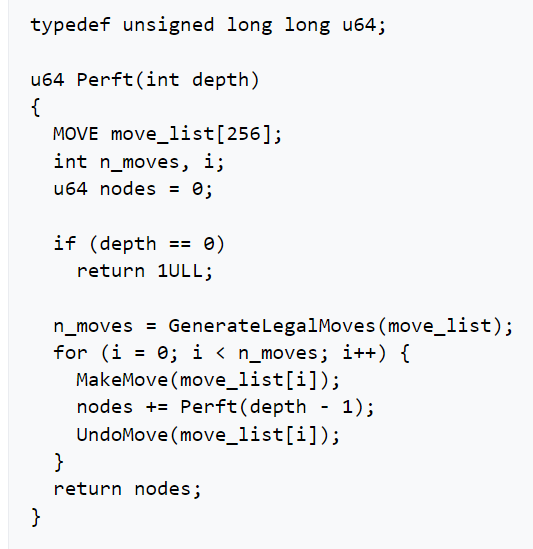
\includegraphics[width=\linewidth/2] {Perft.png}
    \caption{codice di una funzione basica di perft}
\end{figure}


